% 第四章 系统总体设计

\chapter{系统总体设计}


\section{系统总体架构}

FreeFlow 采用桌面端、链下服务、智能合约与 IPFS 存储协同的整体架构。桌面端负责用户交互、钱包连接、播放控制与本地缓存；后端负责认证、上传代理、资源索引、购买记录与评论服务；智能合约负责作品发布、访问授权与收益分账；IPFS/Pinata 负责音频、封面与 metadata 资源存储。系统总体架构如图\ref{fig:system_architecture}所示。

在职责划分上，作品发布结果、访问凭证、交易记录等关键状态由链上维护，评论、会话、搜索索引和上传记录等高频业务数据由链下维护。该分层方式能够在链上可信记录与链下处理效率之间形成较稳妥的工程折中，并降低链上应用在同步、成本和交互延迟方面的实现压力\cite{Wei2022BDMSSurvey,Six2022DAppPatterns}。

\begin{figure}[H]
    \centering
    
\includegraphics[width=\textwidth]{figures/out/system_architecture.png}
    \caption{FreeFlow系统总体架构图}
    \label{fig:system_architecture}
\end{figure}


\section{功能模块设计}

系统模块围绕发布、检索、访问与播放四条主线展开，模块划分如表\ref{tab:module_design}所示。

\begin{table}[htbp]
    \linespread{1.5}
    \zihao{5}
    \songti
    \centering
    \caption{系统功能模块设计}\label{tab:module_design}
    \begin{tabular}{|l|p{10cm}|}
        \hline
        模块        & 设计说明                                           \\ \hline
        用户资料与认证模块 & 使用SIWE完成钱包登录，并在后端创建用户、钱包身份和会话                  \\ \hline
        创作者工作台模块  & 管理发行草稿、作品信息、发布阶段、素材状态和链上发布结果                   \\ \hline
        素材上传模块    & 经后端将音频、封面和metadata上传到Pinata，并保存StorageObject   \\ \hline
        链上发布模块    & 调用PlatformHub发布作品，解析事件并回写tokenId、splitter和交易哈希 \\ \hline
        资源检索模块    & 检索已发布链上音乐资源，并基于排序算法返回可解释结果                     \\ \hline
        购买访问模块    & 查询销售配置、调用buyAccess、记录购买交易并验证访问凭证               \\ \hline
        播放缓存模块    & 通过音频代理支持IPFS gateway音频播放、Range请求和本地缓存          \\ \hline
        评论模块      & 支持用户查看和发布作品评论                                  \\ \hline
    \end{tabular}
\end{table}


\section{业务流程设计}

\subsection{创作者发布流程}

创作者发布流程如图\ref{fig:release_workflow}所示。该流程从发行草稿创建开始，依次完成素材上传、 metadata 生成、链上发布与链上信息缓存。媒体资源由 IPFS 保存，链上记录 metadata URI、访问配置与发行结果等关键状态。

\begin{figure}[H]
    \centering
    
\includegraphics[width=\textwidth]{figures/out/release_workflow.png}
    \caption{创作者链上音乐发布流程图}
    \label{fig:release_workflow}
\end{figure}

创作者发布流程的主要步骤如下：

\begin{enumerate}
    \item 用户连接钱包并完成SIWE登录。
    \item 创作者创建并编辑发行草稿。
    \item 系统上传音频、封面与metadata，并保存CID。
    \item 客户端调用\texttt{PlatformHub}发布作品。
    \item 交易确认后，系统回写\texttt{tokenId}、分账合约地址、交易哈希与区块信息。
\end{enumerate}

\subsection{用户购买播放流程}

用户购买播放流程如图\ref{fig:purchase_playback_sequence}所示。系统先基于链下索引提供检索与详情展示，再以链上状态完成访问资格确认，最后进入播放或下载链路。

\begin{figure}[H]
    \centering
    
\includegraphics[width=\textwidth]{figures/out/purchase_playback_sequence}
    \caption{用户购买与播放流程图}
    \label{fig:purchase_playback_sequence}
\end{figure}

用户购买播放流程的主要步骤如下：

\begin{enumerate}
    \item 用户检索并查看链上音乐资源。
    \item 客户端读取销售配置和访问状态。
    \item 公开作品可直接播放，付费作品需调用\texttt{buyAccess}完成购买。
    \item 访问校验通过后，作品加入链上音乐库并进入播放或下载流程。
\end{enumerate}


\section{数据库设计}

系统采用客户端SQLite数据库与服务器PostgreSQL数据库的双数据库方案。前者用于本地音乐管理、缓存与播放状态维护，后者用于身份认证、资源索引、上传记录、购买记录与评论存储。

\subsection{客户端SQLite数据库设计}

客户端 SQLite 数据库以统一歌曲记录为核心，其 ER 关系如图\ref{fig:client_sqlite_er}所示。

\begin{figure}[htbp]
    \centering
    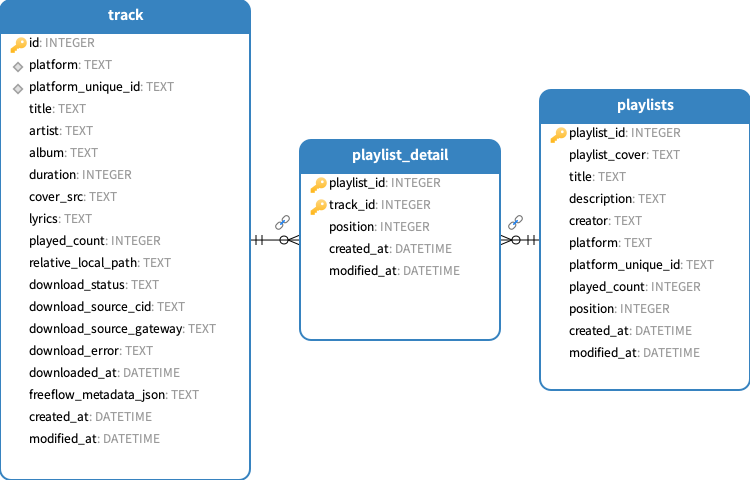
\includegraphics[width=0.95\textwidth]{figures/out/client_sqlite_er.png}
    \caption{客户端SQLite数据库ER图}
    \label{fig:client_sqlite_er}
\end{figure}

客户端SQLite数据库中的核心数据表及其职责如表\ref{tab:client_sqlite_tables}所示。

\begin{table}[htbp]
    \linespread{1.5}
    \zihao{5}
    \songti
    \centering
    \caption{客户端SQLite核心数据表说明}\label{tab:client_sqlite_tables}
    \begin{tabular}{|l|p{10cm}|}
        \hline
        数据表              & 设计说明                                                                \\ \hline
        track            & 保存统一歌曲记录，包括平台标识、平台内唯一ID、标题、歌手、专辑、封面、播放次数、本地文件路径、下载状态和FreeFlow链上扩展信息 \\ \hline
        playlists        & 保存用户歌单信息，包括标题、描述、封面、创建者、来源平台、播放次数和排序位置                              \\ \hline
        playlist\_detail & 保存歌单与歌曲的多对多关系，以playlist\_id和track\_id作为联合主键，并记录歌曲在歌单中的排序位置          \\ \hline
        sessions         & 保存应用启动会话，包括启动时间、操作系统和应用版本，用于记录桌面端运行情况                               \\ \hline
    \end{tabular}
\end{table}

\subsection{服务器PostgreSQL数据库设计}

服务器PostgreSQL数据库的ER关系如图\ref{fig:server_postgresql_er}所示。后端以\texttt{creator\_releases}为资源索引中心，关联用户、钱包身份、存储对象、购买记录与评论数据，以实现资源检索、详情展示、阶段恢复和交易投影等业务需求。

\begin{figure}[htbp]
    \centering
    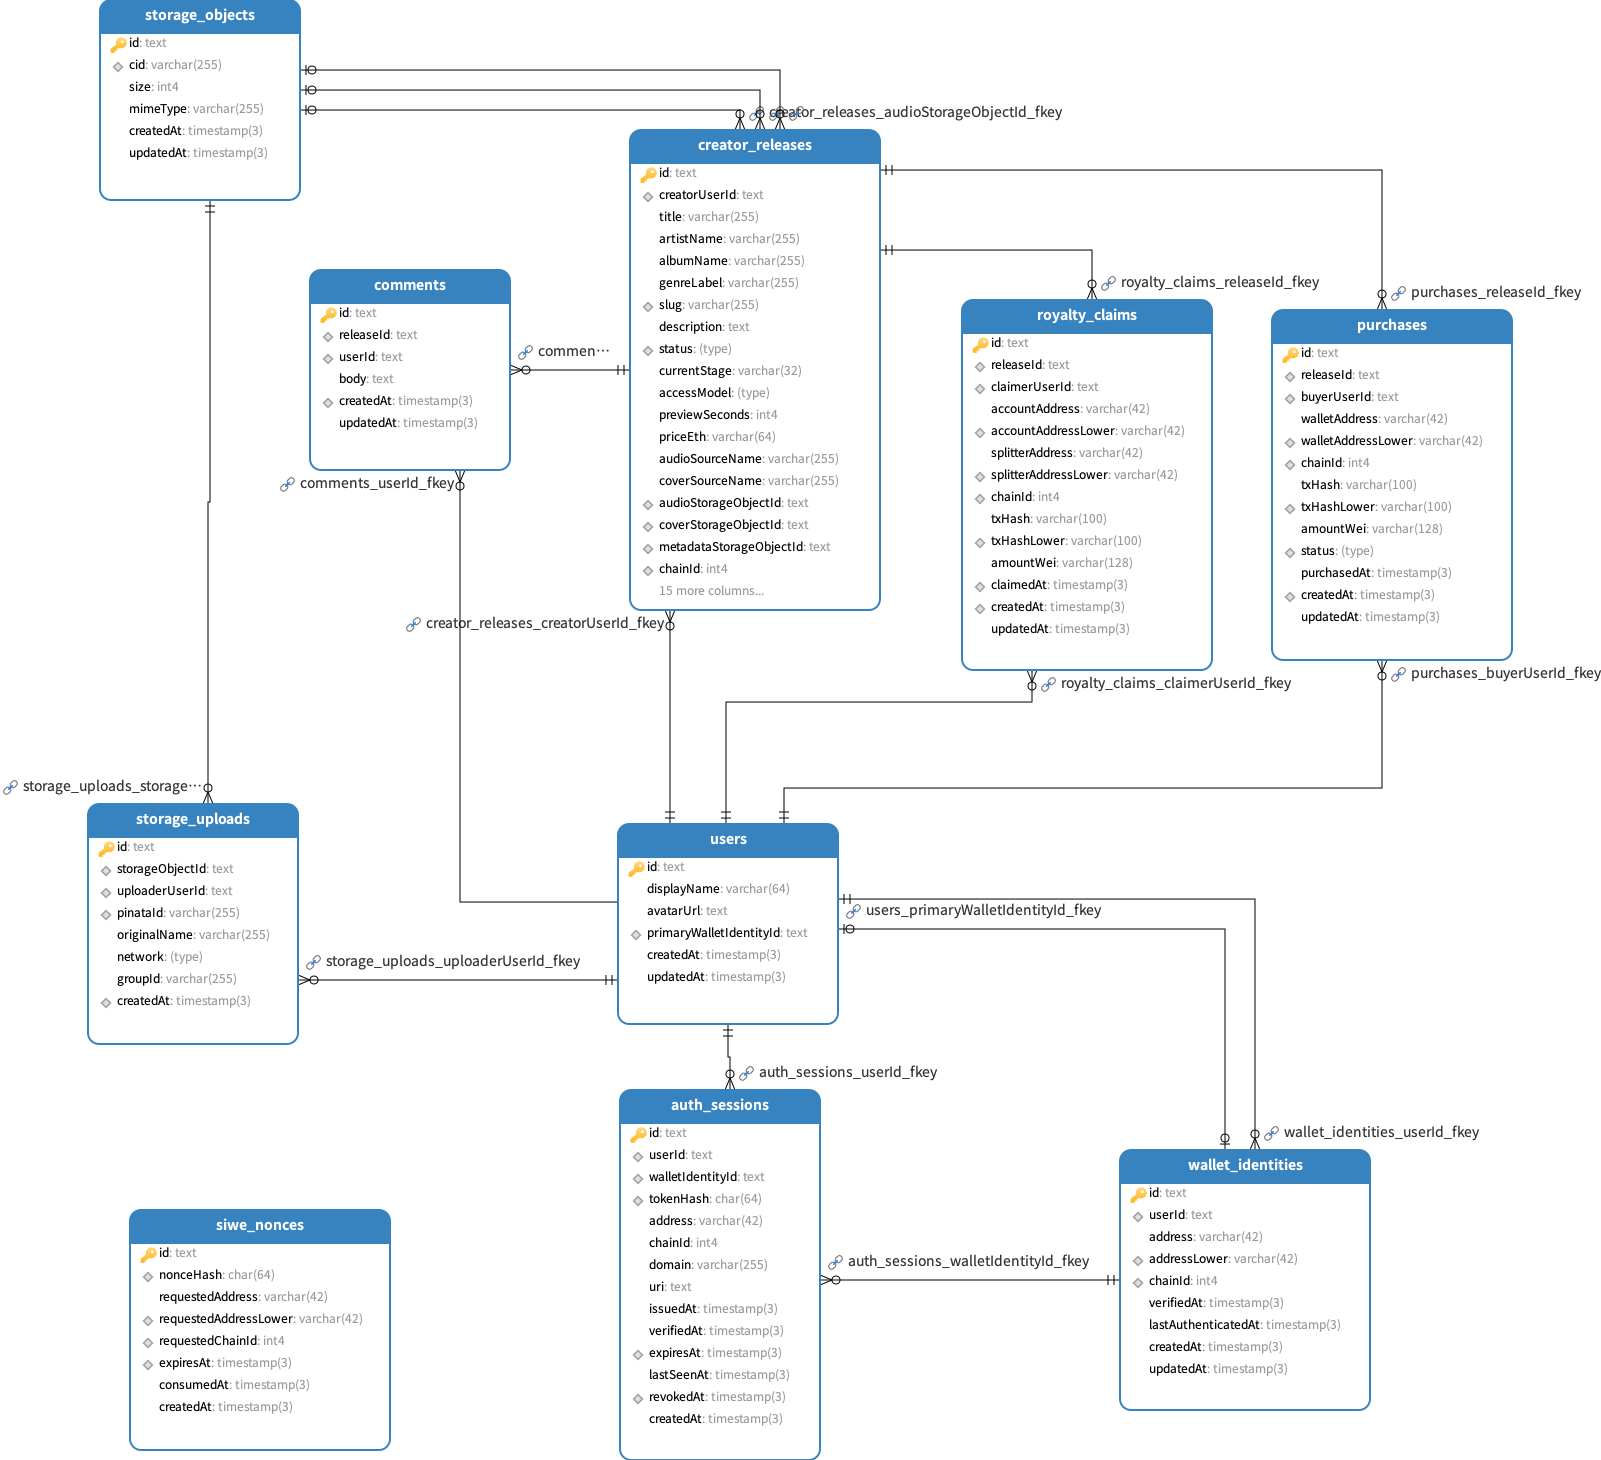
\includegraphics[width=0.98\textwidth]{figures/out/server_postgresql_er.png}
    \caption{服务器PostgreSQL数据库ER图}
    \label{fig:server_postgresql_er}
\end{figure}

服务器PostgreSQL数据库中的核心数据表及其职责如表\ref{tab:server_postgresql_tables}所示。

\begin{table}[htbp]
    \linespread{1.5}
    \zihao{5}
    \songti
    \centering
    \caption{服务器PostgreSQL核心数据表说明}\label{tab:server_postgresql_tables}
    \begin{tabular}{|l|p{10cm}|}
        \hline
        数据表                & 设计说明                                                       \\ \hline
        users              & 保存系统用户资料，包含展示名、头像和主钱包身份引用                                  \\ \hline
        wallet\_identities & 保存钱包地址、链ID、验证时间和用户绑定关系，并通过addressLower与chainId保证同一链上地址唯一   \\ \hline
        siwe\_nonces       & 保存SIWE登录nonce哈希、请求地址、请求链ID、过期时间和消费时间，用于防止签名重放              \\ \hline
        auth\_sessions     & 保存登录会话token哈希、钱包身份、domain、uri、签发时间、验证时间、过期时间和吊销时间          \\ \hline
        storage\_objects   & 保存IPFS/Pinata对象的CID、文件大小和MIME类型，是音频、封面和metadata对象的统一记录     \\ \hline
        storage\_uploads   & 保存上传行为，关联上传者、存储对象、Pinata ID、原始文件名、存储网络和上传时间                \\ \hline
        creator\_releases  & 保存创作者发行项目和链上资源索引，包括作品元数据、发布阶段、访问模式、CID引用、合约地址、tokenId和交易哈希 \\ \hline
        purchases          & 保存购买交易投影，关联发行资源和购买用户，并用交易哈希、钱包地址、链ID等字段避免重复记录              \\ \hline
        comments           & 保存作品评论，关联发行资源和评论用户，并记录评论正文和时间信息                            \\ \hline
    \end{tabular}
\end{table}

\section{智能合约设计}

系统合约由\texttt{MusicAccess1155}、\texttt{PlatformHub}和\texttt{RoyaltySplitter}组成，其结构如图\ref{fig:contract_architecture}所示。\texttt{MusicAccess1155}负责访问凭证创建与校验；\texttt{PlatformHub}负责作品发布、销售配置维护、购买处理与访问状态判断；\texttt{RoyaltySplitter}负责收益保存与提取。

\begin{figure}[htbp]
    \centering
    \includegraphics[width=0.95\textwidth]{figures/out/contract_architecture}
    \caption{智能合约结构图}
    \label{fig:contract_architecture}
\end{figure}

在发布流程中，\texttt{PlatformHub}为作品创建新的\texttt{tokenId}并关联分账合约；在购买流程中，合约校验支付金额与销售配置，随后铸造访问凭证并完成收益分配。各合约职责如表\ref{tab:contract_design}所示。

\begin{table}[htbp]
    \linespread{1.5}
    \zihao{5}
    \songti
    \centering
    \caption{智能合约职责说明}\label{tab:contract_design}
    \begin{tabular}{|l|p{10cm}|}
        \hline
        合约              & 职责                                    \\ \hline
        MusicAccess1155 & 为每首作品创建ERC-1155 tokenId，购买者持有不可转让访问凭证 \\ \hline
        PlatformHub     & 统一发布作品、保存销售配置、处理购买、判断访问状态和收取平台费       \\ \hline
        RoyaltySplitter & 按固定份额保存创作者和协作者收益，支持按地址提取              \\ \hline
    \end{tabular}
\end{table}


\section{系统安全设计}

系统安全设计主要集中在身份建立、访问控制、接口保护以及资源访问边界几个方面。本系统使用 SIWE 签名登录机制，后端会对 nonce、地址、链 ID、domain、uri 和签发时间等进行校验并恢复出钱包地址并与传入地址比对，nonce 具有过期时间和消费限制，以防范重放攻击。

在访问控制方面，创作者可将作品发布为“公开可访问”或“购买后访问”。前端以链上信息为唯一事实，通过静态调用来获取链上状态，从而能够在链上形成一种可公开查验的确权模式\cite{Maesa2019AuditableAC,Qin2021BlockchainAccess,Punia2024AccessReview}。

在资源保护上，当前模式下，如果资源地址被直接获取，仍有可能绕过应用这边的访问流程。已经有研究表明，链上与链下的混合去中心化应用架构中，链上的确权信息仍需配合链下的加密、密钥管理或类似 Lit Protocol 等去中心化鉴权模式才能有效防止盗链\cite{Ali2017IoTIPFS,Qin2021BlockchainAccess}。现阶段的访问控制，只是原型系统的授权验证机制，后续需要结合音频加密、授权网关来完善资源保护。
